
\documentclass[fleqn,addpoints]{exam}

\usepackage{graphicx}
\usepackage{float}
\usepackage{amsmath}
\usepackage{cancel}
\usepackage{polynom}
\usepackage{caption}
\usepackage{mdwlist}

\printanswers

%% \ifprintanswers 
%% \usepackage{2in1, lscape} 
%% \fi

\title{Math 115 \\ Homework 19}
\date{April 19, 2011}

\begin{document}

\maketitle

% \begin{figure}[H]
%   \centering
%   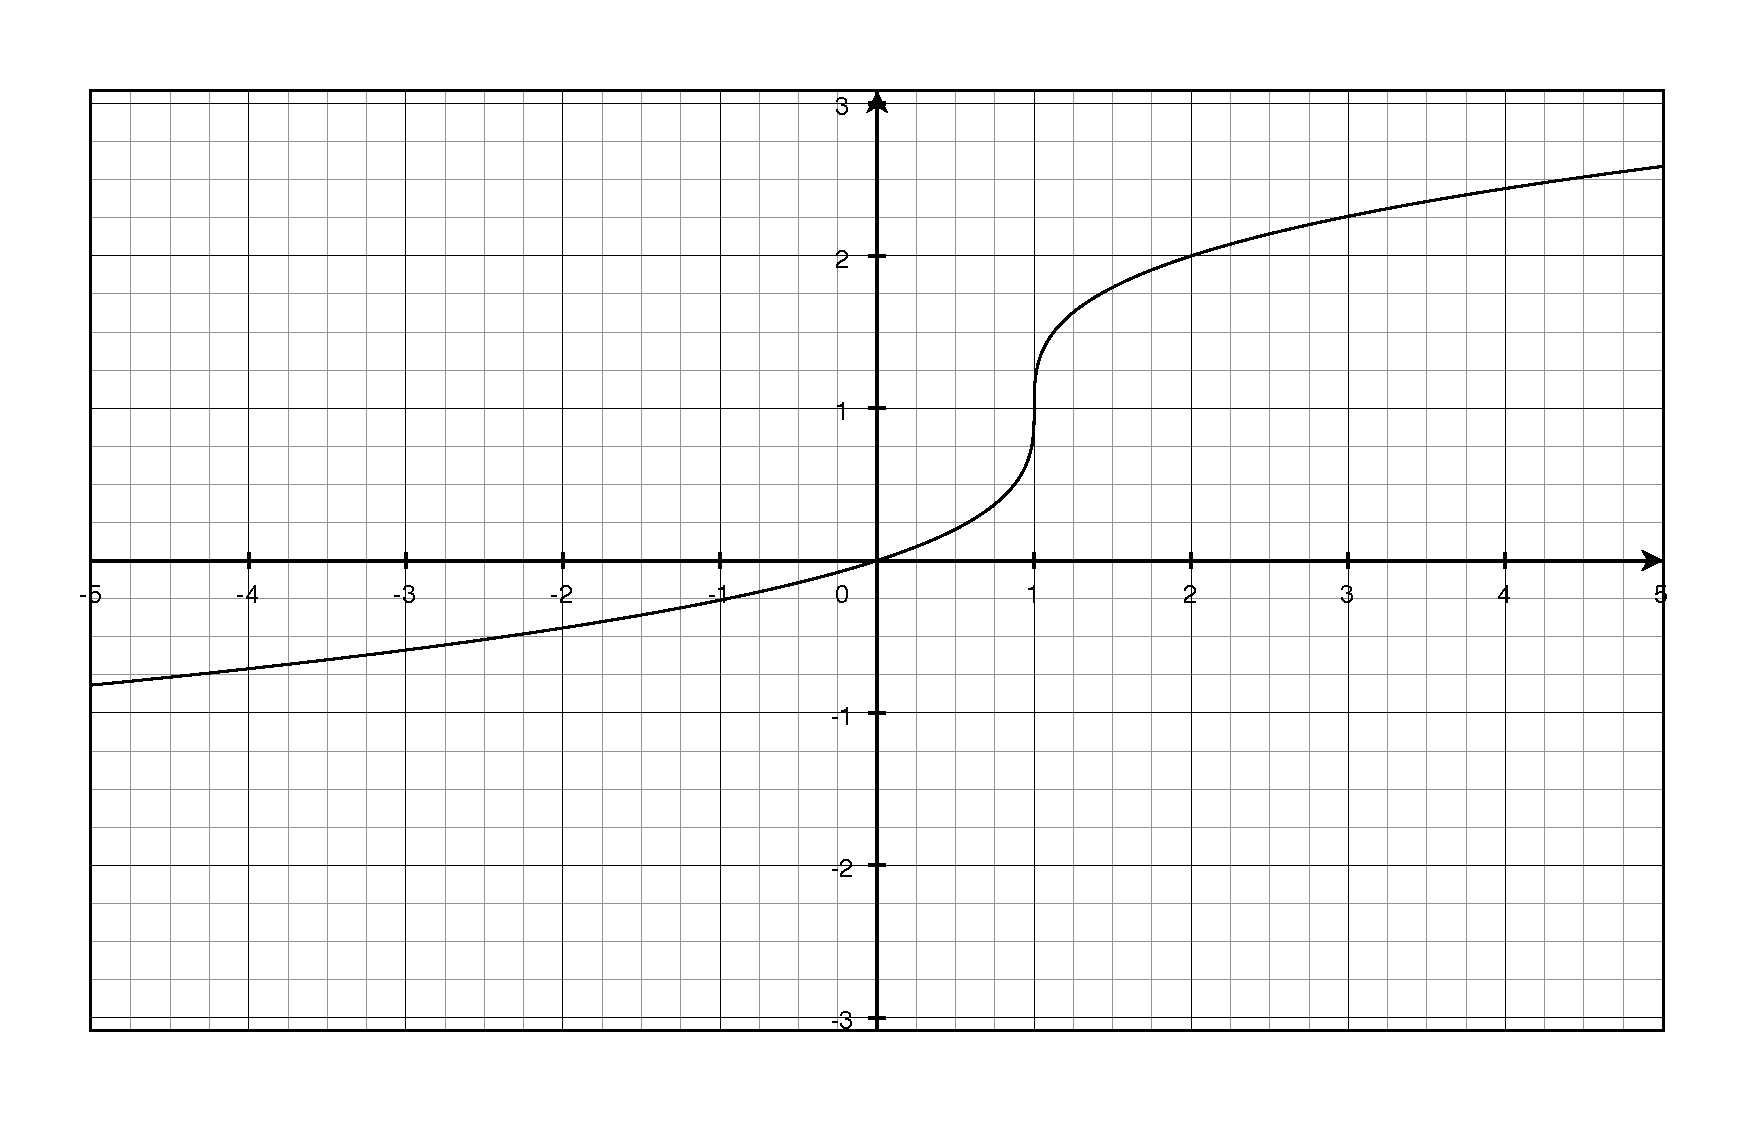
\includegraphics[scale=.3]{question7.eps}
%   \caption*{Question 7}
% \end{figure}

\ifprintanswers
\else
\section{Review}

To make sure you remember how to do all the things we've covered so far, you might want to do the {\em Cumulative Test
  for Chapters 1.3} on pp. 348-49, but you don't have to hand it in.  
\fi

\section{Extra Credit}

Two ferryboats start at the same instant from opposite sides of a river, traveling across the water on routes at right
angles to the shores.  Each travels at a constant speed, but one is faster than the other.  They pass at a point 720
yards from the nearest shore.  Both boats remain in their slips for 10 minutes before starting back.  On the return
trips they meet 400 yards from the other shore.

How wide is the river?

\begin{solution}[4 in]
The key point for this problem is that the ratio between the distances traveled is always the same as the ratio of the
speeds of the boats.  If the fast boat is going twice as fast as the slow boat, it has always gone twice as far. 

There are two points where we know the distances.  At the first point, the slow boat has traveled 720 yards from its
starting point and the fast boat is 720 yards away from the slow boat's dock.  We know that this is the situation
because the boats are 720 yards from the nearest shore and they must be closer to the slow boat's shore.  If $x$ is the
width of the river, this gives us these two equations:
\begin{itemize*}
  \item slow boat distance traveled = 720
  \item fast boat distance traveled = x - 720
\end{itemize*}

At the second point, the slow boat has docked and started back.  It is now 400 yards into its return trip and has
traveled the width of the river plus 400 yards.  The fast
boat is nearly done.  It is only 400 yards away from its starting point and is just 400 yards short of traveling the
width of the river twice.  This gives us these two equations:
\begin{itemize*}
  \item slow boat distance traveled = x + 400
  \item fast boat distance traveled = 2x - 400
\end{itemize*}

Since the ratio of the distances is constant, the ratio must be the same at both points.  So we just need to solve this
equation:

\begin{align*}
  \frac{720}{x-720} &= \frac{x+400}{2x-400} \\
  1440x - 288000 &= x^2 -320x - 288000 \\
  1440x &= x^2 -320x \\
  x^2 - 1760 &= 0 \\
  x(x-1760) &= 0 \\
\end{align*}

x is either 0 or 1760.  But 0 doesn't make sense for a river width, so the only solution is 1760 yards.

\end{solution}

\ifprintanswers
\else
{\em I am as desirous of being a good neighbor as I am of being a bad subject.}

\vspace{.1 cm}
\hspace{1 cm} --Henry David Thoreau

\fi

\end{document}

